\documentclass[12pt]{article}
\usepackage[english]{babel}
\usepackage[utf8x]{inputenc}
\usepackage{amsmath}
\usepackage{tikz}
\usetikzlibrary{arrows,automata}
\begin{document}

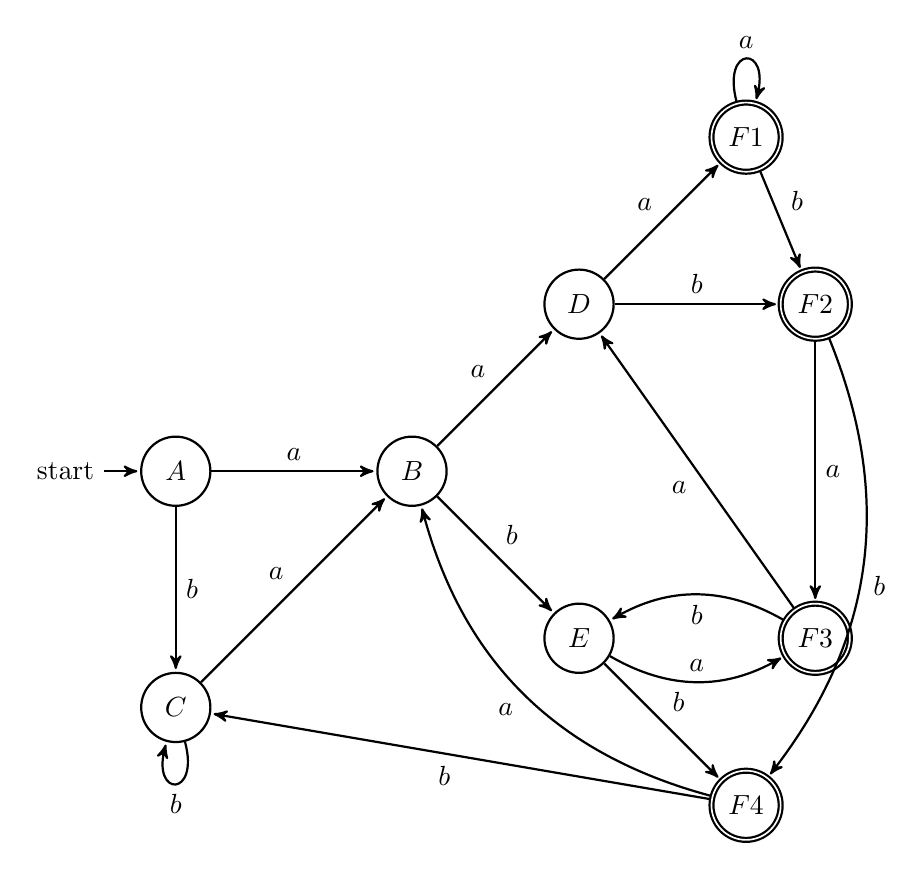
\begin{tikzpicture}[->,>=stealth',shorten >=1pt,auto,node distance=3cm,
    thick,base node/.style={circle,draw,minimum size=8pt}, real node/.style={double,circle,draw,minimum size=17pt}]

  \node[state,initial]          (a) {$A$};
  \node[state]                  (b) [right of=a] {$B$};
  \node[state]                  (c) [below of=a] {$C$};
  \node[state]        (d) [above right of=b]   {$D$};
  \node[state]        (e) [below right of=b]  {$E$};
  \node[state,accepting]        (f1) [above right of=d]  {$F1$};
  \node[state,accepting]        (f2) [right of=d]  {$F2$};
  \node[state,accepting]        (f3) [right of=e]  {$F3$};
  \node[state,accepting]        (f4) [below right of=e]  {$F4$};
  \path (a) edge       node {$a$} (b)
        (a) edge       node {$b$} (c)
        (b) edge       node {$a$} (d)
        (b) edge       node {$b$} (e)
        (c) edge       node {$a$} (b)
        (c) edge  [loop below]     node {$b$} (c)
        (d) edge       node {$a$} (f1)
        (d) edge       node {$b$} (f2)
        (e) edge  [bend right]     node {$a$} (f3)
        (e) edge       node {$b$} (f4)
        (f1) edge  [loop above]     node {$a$} (f1)
        (f1) edge       node {$b$} (f2)
        (f2) edge       node {$a$} (f3)
        (f2) edge   [bend left]    node {$b$} (f4)       
        (f3) edge       node {$a$} (d)
        (f3) edge   [bend right]    node {$b$} (e)    
        (f4) edge  [bend left]     node {$a$} (b)
        (f4) edge       node {$b$} (c)    
        
        
        ;

\end{tikzpicture}
\end{document}